\documentclass{article}

\usepackage{arxiv}

\usepackage[utf8]{inputenc} % allow utf-8 input
\usepackage[T1]{fontenc}    % use 8-bit T1 fonts
\usepackage{hyperref}       % hyperlinks
\usepackage{url}            % simple URL typesetting
\usepackage{booktabs}       % professional-quality tables
\usepackage{amsfonts}       % blackboard math symbols
\usepackage{nicefrac}       % compact symbols for 1/2, etc.
\usepackage{microtype}      % microtypography
\usepackage{cleveref}       % smart cross-referencing
\usepackage{lipsum}         % Can be removed after putting your text content
\usepackage{graphicx}
\usepackage{natbib}
\usepackage{doi}

\title{Sweet-Gossip - P2P protocol for the \emph{GIG} economy}

% Here you can change the date presented in the paper title
\date{January 19, 2023}
% Or remove it
%\date{}

\author{
	{Sonof Satoshi}\thanks{We are the children of Nakamoto} \\
	Public Key (GPG)~\ref{gpgkey} \\
	\href{www.donttrustverify.org}{Dont Trust, Verify}\\
	www.donttrustverify.org \\
	\texttt{sonof.satoshi@donttrustverify.org}\\
}

% Uncomment to override  the `A preprint' in the header
%\renewcommand{\headeright}{Technical Report}
%\renewcommand{\undertitle}{Technical Report}
\renewcommand{\shorttitle}{\textit{Sweet-Gossip} Protocol}

%%% Add PDF metadata to help others organize their library
%%% Once the PDF is generated, you can check the metadata with
%%% $ pdfinfo template.pdf
\hypersetup{
pdftitle={Sweet-Gossip - P2P protocol for the GIG economy},
%%%pdfsubject={q-bio.NC, q-bio.QM},
pdfauthor={Sonof Satoshi},
pdfkeywords={GIG Economy, Gossip Protocol, Distributed System, P2P, Bitcoin, Lightning Network, BTC, LND},
}

\begin{document}
\maketitle

\begin{abstract}
Sweet-Gossip protocol is a P2P, mobile-first, Proof of Work protected, gossip protocol built on top of the Lightning Network that enables message broadcast (job proposal) and replies (job offer). It uses a game-theoretic approach to preserve its properties that are aligned with the Bitcoin ecosystem.
\end{abstract}


% keywords can be removed
\keywords{GIG Economy \and Gossip Protocol \and Distributed System \and P2P Network\and Bitcoin \and Lightning Network}


\section{Motivation}

GIG economy refers to the work done by casual workers coordinated by a software system. At the time of this writing, the end-customer of the Gig economy directly interacts with the centralized, cloud-based platform (app). This platform is also used to pay for the services after the job is done to the platform, which in turn is sharing the revenue with the assigned GIG worker. The actual job is done by the GIG worker for their customer, making the online platform a tool that supports and manages the effectiveness of the job.

This kind of cybernetic system uses the human power of GIG workers managed by AI, to extract value for the company shareholders. The AI component of the platform uses behavioural data represented as all the user (both GIG workers and customers) interactions with the platform to maximize the total revenue generated by the system and the underlying company that operates it. To optimise the global goal, which is the company revenue, the platform is implementing gamification and for-purpose misinformation techniques. It is possible because GIG workers and customers have no other option but to trust the platform for its efficiency and the underlying operation of the platform is opaque to users and configurable only by the operating central company. Therefore the platform operator:

\begin{enumerate}
\item dictates the revenue sharing and can change this anytime dependingly on the socioeconomic circumstances without giving any reason to GIG workers

\item punish workers that are not behaving properly, that is aligned with company benefit, e.g. by blocking them from access to the platform
\end{enumerate}

We are proposing a P2P protocol designed for the Gig economy that, by eliminating the need for central online platforms, will create a new decentralized, P2P GIG economy. Gig workers will be engaged directly by the end customer and can accomplish their tasks and earn money on a free market without the need for the existence of a central organization or any other trusted third party.

Lack of central organization also means that a minimal volume of data is shared between GIG workers and end-customers, just enough to fulfil the job according to the protocol-driven off-chain smart contract that uses P2P money i.e. Lightning Network \cite{poon2016bitcoin} on Bitcoin \cite{nakamoto2009bitcoin}, therefore forming layer 3 protocol from the Bitcoin perspective.

\section{Sweet-Gossip P2P Network}
Sweet-Gossip P2P Network is a global, symmetric, P2P network, meaning that there is no direct need to run any operation critical services in the cloud or any other centralised computing environment. Sweet-Gossip node is a software module that is run by every device that uses Sweet-Gossip protocol and forms a basis of communication. Sweet-Gossip nodes can be implemented as apps and run efficiently on cheap modern mobile devices. The need for implementation of supporting services that are cloud-based or edge-computing-based helps make the service more user-friendly but is never critical for the network operation.

It is important to state explicitly that we are not inventing any new coin or crypto token, but rather we are speaking about how Sweet-Gossip protocol forms a layer 3 protocol on top of the Lightning Network (being itself a layer 2 network sitting on top of Bitcoin network), therefore if any, the Bitcoin is a native token of the Sweet-Gossip Network.

Sweet-Gossip P2P Network preserves:
\begin{itemize}
\item P2P Symmetry - every node does the same thing
\item Permissionlessness - anyone with internet access can join Sweet-Gossip P2P network
\item Mobile first - the cost of running Sweet-Gossip node is marginal on modern mobile devices. Also, the protocol handles mobile connectivity issues.
\item Privacy - the communication is encrypted
\item Anonymity - any personal information about the people behind the nodes is hidden
\item DDos and Spam protection - it uses Proof of Work (PoW) and/or micropayments to protect the network from DDoS and Spam
\item Sustainability - the protocol is designed so all its participants benefit from joining the network
\item Implicit punishment - the protocol do not explicitly punish unhonest participants, but rather makes honest participant benefit more than unhonest ones
\end{itemize}

Sweet-Gossip Protocol is a gossip protocol \cite{Fanout}, that allows a network to broadcast in a similar way to gossip spreads. Assuming that each sweet-gossip node is connected to its peers and that the network graph is connected, each node works independently and in the event of receiving a message that needs to be broadcasted. It selects several peers and sends the message, in its owner's interest, to peers making the message spread over the network like gossip (Figure~\ref{fig:network}). There inevitably occurs a situation that, if some node will not send the message to all of its peers, some nodes will not receive a broadcasted message even if a network graph is connected (e.g. node C on Fig 1.), but from the game theoretic perspective it will not be a beneficial situation, so this is up to the network operators to make the flow as efficient as possible.

Sweet-Gossip is a protocol, meaning that it only specifies the minimal set of rules to make it beneficial for all the nodes. It doesn't say explicitly how the network node should be implemented. The node implementation is free to do whatever is best to make it beneficial for the node owner.

\begin{figure}
	\centering
	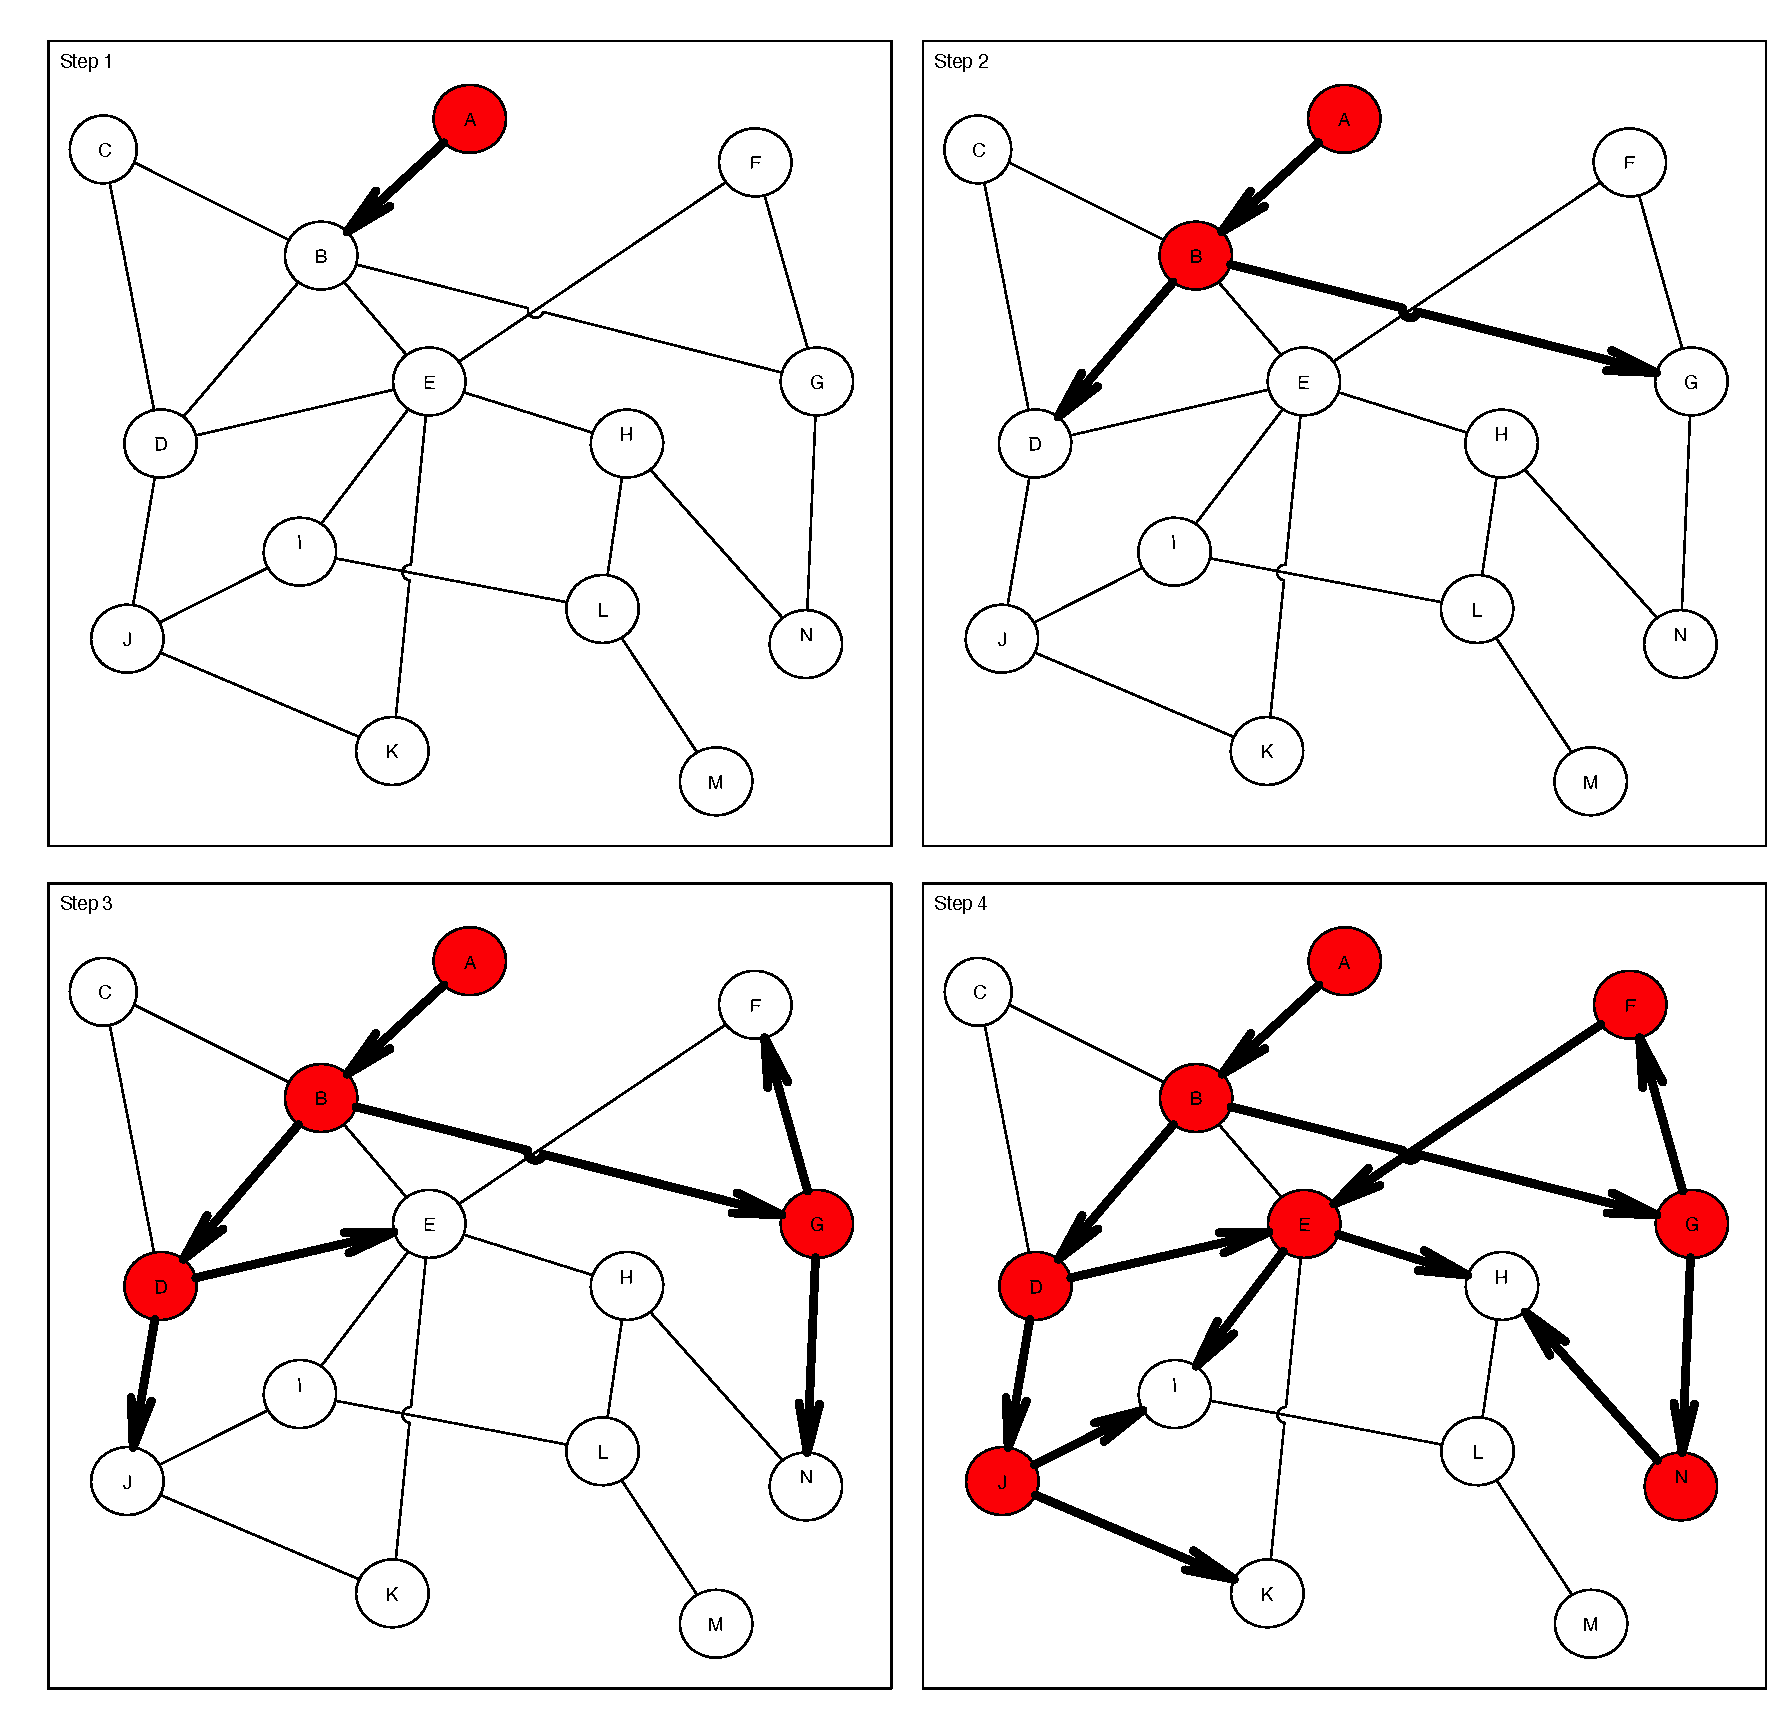
\includegraphics[scale=0.4]{network.pdf}
	\caption{The intuition behind gossip protocol}
	\label{fig:network}
\end{figure}

\section{The protocol}

Sweet-Gossip protocol has a single purpose: to broadcast a job proposal (topic) to interested parties and collect job offers (reply messages) from interested contractors. Economicly, the customer is interested in exchanging their money for the service, while gig-worker is interested in being paid for the job done. The network to sustain its existance needs to reward broadcasters for quality of the broadcasting. Therefore the protocol is constructed in a way that the customer broadcasts a topic, that contains anonymous job description. This job description is delivered by the network to the gig-worker that respond with network encrypted reply message. The message is delivered back to the customer that can verify basic properties of the gig-worker with their digital certificate but to decrypt contact information of the gig-worker is obligated to pay the network.

For sake of clarity we use the following naming convention:

\begin{enumerate}
	\item Topic - the job proposal broadcasted through the network
	\item Reply Message - the job offer for specific topic sent from the contractor
	\item Peer - any gossip network node. Every peer maintains a list of their peers.
	\item Sender - Peer that is the source of the topic. From the Gig economy point of view, it is a customer.
	\item Originator - Peer that is currently broadcasting the topic to the its peers.
	\item Middleman - Peer that is passing the broadcasted topic further as well as bringing back the reply message
	\item Replier - Peer that is replying to the broadcasted topic with reply message.
\end{enumerate}

We assume that nodes of the sweet-gossip network are already connected to their peers via some internet transport protocol (e.g. TCP, UDP with or without hole punching \cite{WebRTC}, mobile mesh etc.) and the other peer is also accepting sweet-gossip protocol. How the nodes discover their peers is not a part of the protocol.

In short the sweet-gossip protocol can be summarised as follows:

\begin{enumerate}
	\item  \textbf{Asking for broadcast} If the originator (e.g. Node A) wants to broadcast the topic first step is to ask its selected peer (e.g. Node B) how about condition of its coopertation. If the middleman accepts this kind of tipics, it replies to the originator with specific POW properties the originator needs to provide to be able to broadcast the topic with using this specific middleman.
	\item  \textbf{Broadcast with POW:} In order to use this middleman the originator must compute hash (e.g. SHA256) that is less or equal to the specific target for the specific POW scheme. The computed POW is passed with the topic to the broadcaster and if the brodcaster validates the hash it brodcast the topic to its peers.
	\item  \textbf{Replying:} If the middleman instead is interested in accepting the job it becomes the replier. Replier constructs the Reply Message. The Reply Message contains all the information that is required to pay for the reply message delivery to all the middlemans involved. The reply message is passed back to the originator
	\item  \textbf{Paying for the reply message:} Once the message reaches the originator, the originator needs to pay the network using the specific payment method. Once paid the reply message is revilled and the originator is able to begin direct communication with replier.
\end{enumerate}

\subsection{Topic}

The topic is a data-structure that defines the basic requirements for the job. It is application specific and by design it should not reveal any information about the originator allowing for their identification.

Lets use a Taxi-app as an example {Figure~\ref{fig:fr:topic}}. The topic of this taxi-app has a form of geohash and time interval describing from where and when the ride can be executed. Geohash here is a way of encoding a specific geographical place (geographical cell that has a form of rectangle) in a form of a string where the lenght of the geohash determines its precision.

\begin{figure}
	\centering
	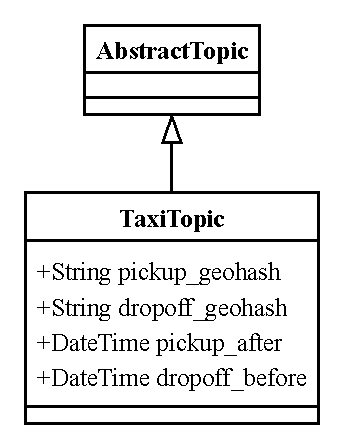
\includegraphics[scale=1.0]{Topic.pdf}
	\caption{The topic frame}
	\label{fig:fr:topic}
\end{figure}


For example Legal Services Counsil in Sydney is located at the following coordinates latitude= -33.8647 and longitude=151.2096 and the corresponding geohash of precision 7 is equal to `r3gx2g5`.

The precision of geohash determines the size of the cell (Table~\ref{tab:geoprec}) and to be useful for the Taxi-app it needs to be atleast 7 so the cell has size lower than 200m (see table below)

\begin{table}
	\centering
	\begin{tabular}{lll}
		\toprule
		Geohash length & Cell width & Cell height \\
		\midrule
		1  & $\le$ 5,000km & $\times$ 5,000km \\
		2  & $\le$ 1,250km & $\times$ 625km   \\
		3  & $\le$ 156km   & $\times$ 156km   \\
		4  & $\le$ 39.1km  & $\times$ 19.5km  \\
		5  & $\le$ 4.89km  & $\times$ 4.89km  \\
		6  & $\le$ 1.22km  & $\times$ 0.61km  \\
		7  & $\le$ 153m    & $\times$ 153m    \\
		8  & $\le$ 38.2m   & $\times$ 19.1m   \\
		9  & $\le$ 4.77m   & $\times$ 4.77m   \\
		10 & $\le$ 1.19m   & $\times$ 0.596m  \\
		11 & $\le$ 149mm   & $\times$ 149mm   \\
		12 & $\le$ 37.2mm  & $\times$ 18.6mm  \\
		\bottomrule
	\end{tabular}
	\caption{Geohash precision}
	\label{tab:geoprec}
\end{table}

On the other hand we dont want to be to specific and we might want to restrict the size of geohash to at most 8, so it is not possible to precisly locate the originator (customer) at this stage, but on the other side the precision is enough for the taxi driver to accept/reject to job.

\subsection{Digital Certificates}

Every gig economy envinronemnt needs to be safe for both customer and gig-worker. Safety means here the ability to have a level of trust that the other party will not violate civil rights of the other part during the service delivery either if it is a giving a ride, delivering food or programming website. The way to implement a physical levels of trust in the internet is done using Digital Certificates implemented as public-key certificate (e.g. X.509 certificates). These certificates are issued by certification authorities that can be either trusted 3rd parties, or communities. For a taxi-driver the minimal certification requires having valid driveing licence and no criminal record. The trusted 3rd party can issue this kind of certificate and by signing it with its private key so anyone can verify that the specific ceriticate was trully issued by this trusted 3rd party. If the certificate is revoked the information about it is published by the trusted 3rd party in form of a revocation list. Public key certificates contain also a public key of the certified person, so it is possible use it to encrypt a message that is targetted for this person and verify their signatures.

\begin{figure}
	\centering
	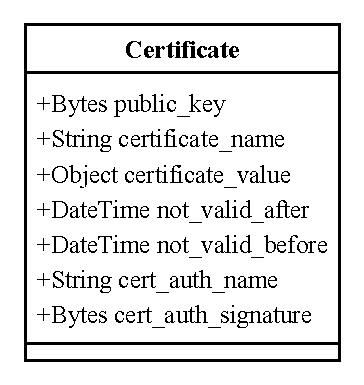
\includegraphics[scale=1.0]{Certificate.pdf}
	\caption{The digital certificate}
	\label{fig:fr:certificate}
\end{figure}


On the other hand we dont want to be to specific and we might want to restrict the size of geohash to at most 8, so it is not possible to precisly locate the originator (customer) at this stage, but on the other side the precision is enough for the taxi driver to accept/reject to job.

\subsection{Asking For Broadcast}
The first step of sweet-gossip protocol is to send the AskForBroadcastFrame to the potencial broadcaster.

\begin{figure}
	\centering
	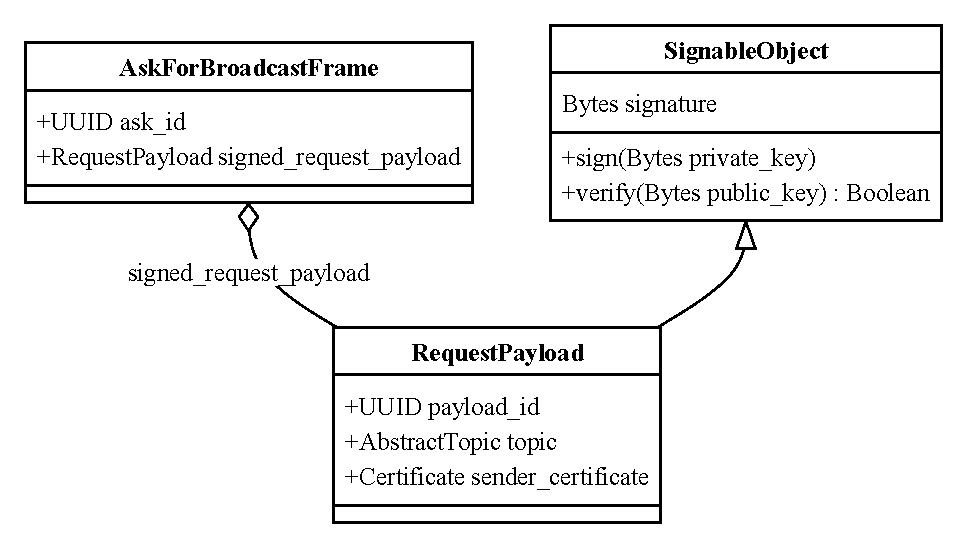
\includegraphics[scale=1.0]{AskForBroadcast.pdf}
	\caption{The Ask For Broadcast Frame}
	\label{fig:fr:askforbroadcast}
\end{figure}

AskForBroadcastFrame contains ask-identifier and digitally signed RequestPayload. signed RequestPayload is made of unique payload\_id, topic (e.g. TaxiTopic), sender certificate and sender signature obtained by signing the RequestPayload with with the sender private key that is complementary to the public key stored withing the sender certificate. Anyone can verify the Request Payload by validating its signature with sender public key from the certificate. Sender certificate can always be verified using  public key of the certification authority and checking its published revocation list.

Ask-identifier allows for the frame identification during the originator-middleman ping-pong communication (see figure below). In the gossip protocol it is possible that the same broadcasting message hits the same gossip node many times, so payload\_id is to remain unique identifier that allows to determine this situation limiting these situations to minimum. It is the requested responsibility to ensure the uniuqueness of payload\_id, risking if it is not unique it will be lost during the broadcast as other nodes can decide that it was already broadcasted if the payload\_id was already seen before.

\begin{figure}
	\centering
	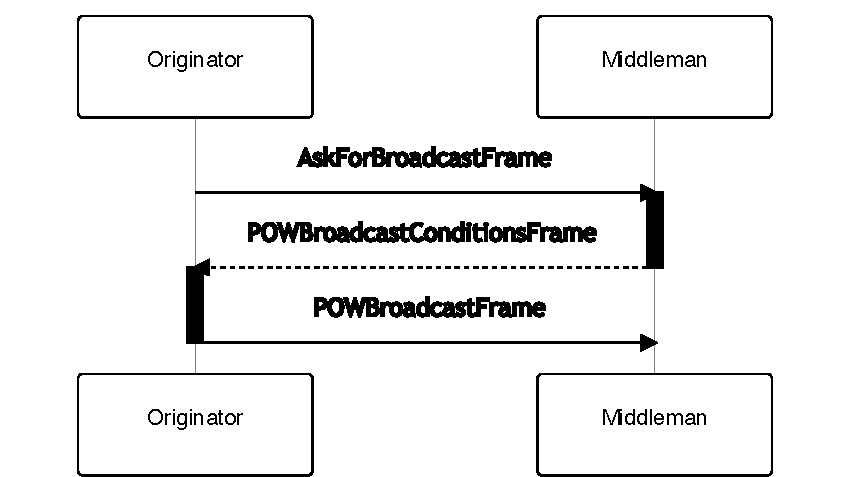
\includegraphics[scale=0.6]{PingPong.pdf}
	\caption{Ping Pong Sequence}
	\label{fig:fr:pingpong}
\end{figure}

\subsection{Proof Of Work (POW)}
Message broadcast in protected in sweet-gossip with the idea of Proof of work, introduced in HashCash \cite{Hashcash} and famously implemented in bitcoin mining but originally introduced to limit the email spam. The thinking here is that if the originator needs to take some significant computational cost to be able to send the message it will significantly reduce the possibility of DDoS attacks. There are many possible POW schemas, here we are considering SHA256 hash based POW, similar to the one implemented in the bitcoin network. In short, given the topic the middleman decides how complex POW is required to be computed by the originator to allow him for further spreading of this topic. The task is to compute the hash of the BroadcastPayload so the hash itself is lower or equal to specific target. The larger target is the more complex the computation become. On the other hand, once the hash is computed, it is easy to verify that it fits into specific target, so the brodcaster has an easy task here to make sure that the originator has done the work to compute the correct hash.

\subsection{Onion-routing}

Sweet gossip is using onion-routing technique to hide the message reply route from the participating middlemen. During the broadcast phase the onion grows layer by layer. Active peer appends its adress to the onion and is using public key of the next peer to encrypt the new onion, therefore only the next peer can decrypt that layer of the onion. Once encrypted the onion is passed to the next peer.

\begin{figure}
	\centering
	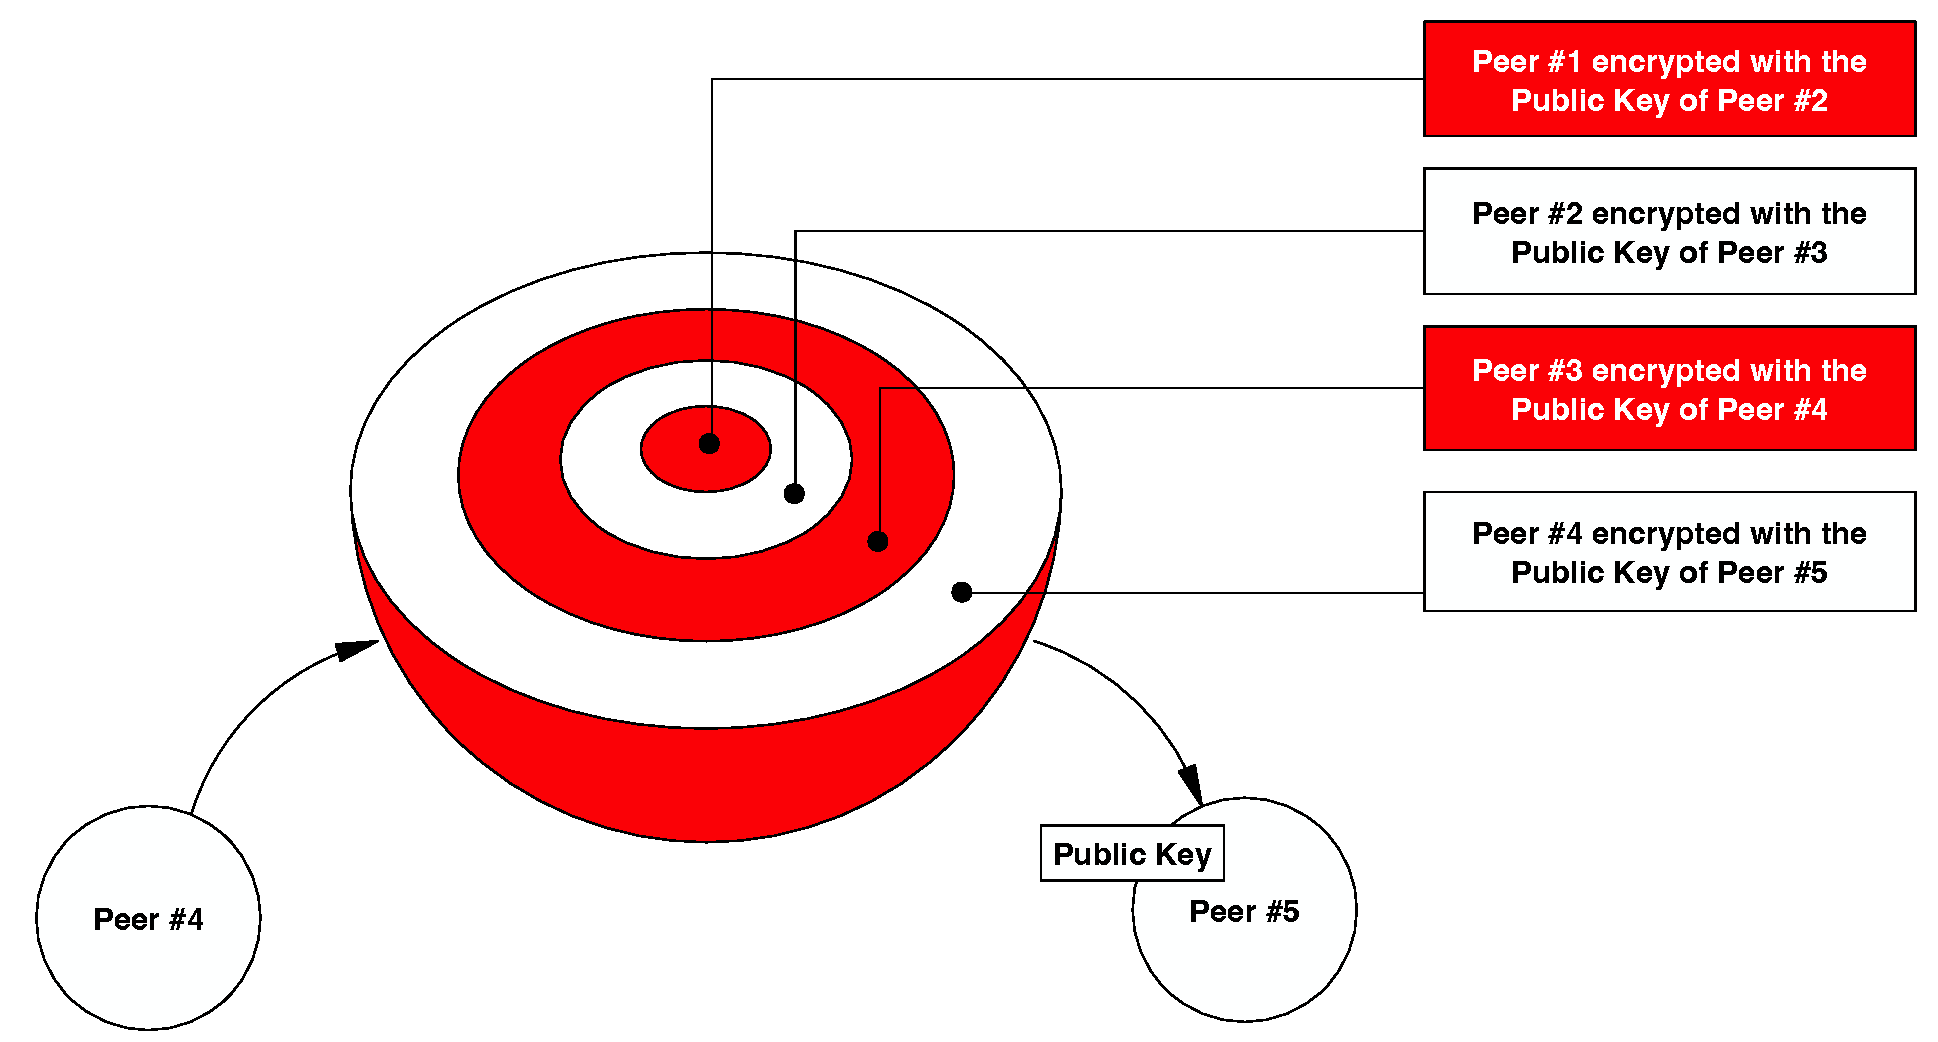
\includegraphics[scale=0.5]{onion.pdf}
	\caption{Onion-routing}
	\label{fig:fr:onionrouting}
\end{figure}

This way of constructing the onion allows then to peel the onion back to the sender through the network in a way that none of the nodes knows the sender nor the distant peers.

\subsection{Broadcast with POW}

If the middleman accepts the topic specified in the AskForBroadcastFrame, it sends back the POWBroadcastConditionsFrame. This frame describes the properties of POW expected to be computed by the originator and payment instructions expected by the peer for delivering the reply.

\begin{figure}
	\centering
	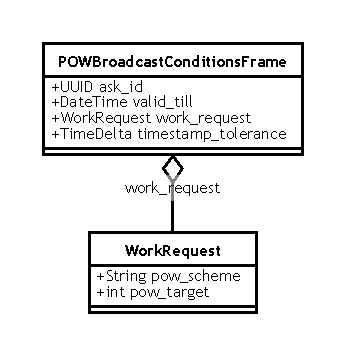
\includegraphics[scale=1.0]{POWBroadcastCondition.pdf}
	\caption{POWBroadcastConditionsFrame}
	\label{fig:fr:powbroadcastcondition}
\end{figure}

Starting with ask\_id, that matches with AskForBroadcastFrame, and valid\_till timeout meaning that the middleman will wait only till the specific time for the POWBroadcastConditionFrame from the originator contains also WorkRequest that describes properties of POW. Routing payment instruction consists of the anonymous account and the amount to be paid. The amount here means only the price for this specific broadcast and the entire price of the reply is given as a sum given by all the middlemen that participate in this gossiping activity.

Originator is replying with POWBroadcastFrame that is also marked with corresponding ask\_id. The main part is a broadcast payload that contains original signed request payload (the one that was a part of AskForBroadcast and was already signed by the originator), onnion-routing and routing payment instructions namely: backward\_onion and routing\_payment\_instruction\_list, both will be discussed here later.

POWBroadcastFrame also contains ProofOfWork that contains a hash value (nuance) that fits below pow\_target for the specific pow\_scheme, and was computed as a hash of broadcast\_payload part, therefore middleman can easly verify nuance value by computing hash of broadcast\_payload and checking if it is lower or equal to the pow\_target.

\begin{figure}
	\centering
	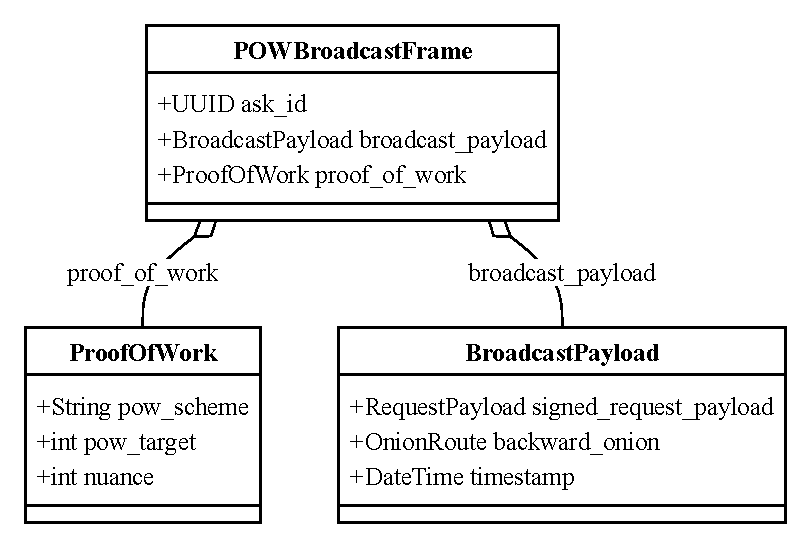
\includegraphics[scale=1.0]{POWBroadcastFrame.pdf}
	\caption{POWBroadcastFrame}
	\label{fig:fr:powbroadcastframe}
\end{figure}


Each step of the broadcast involves passing specific Broadcast Payload that consists of Request Payload that is never changed and protected by the cryptographic signature.  Additionally, every Broadcast Payload has growing routing payment instruction list as well as adds new layer to the onion.

In the gossip protocol nodes are randomly selected from the list of all the known peers of the originator. This number is sometimes refered as fanout \cite{Fanout} of the gossip protocol. Once selected the broadcasting process is performed.

\begin{figure}
	\centering
	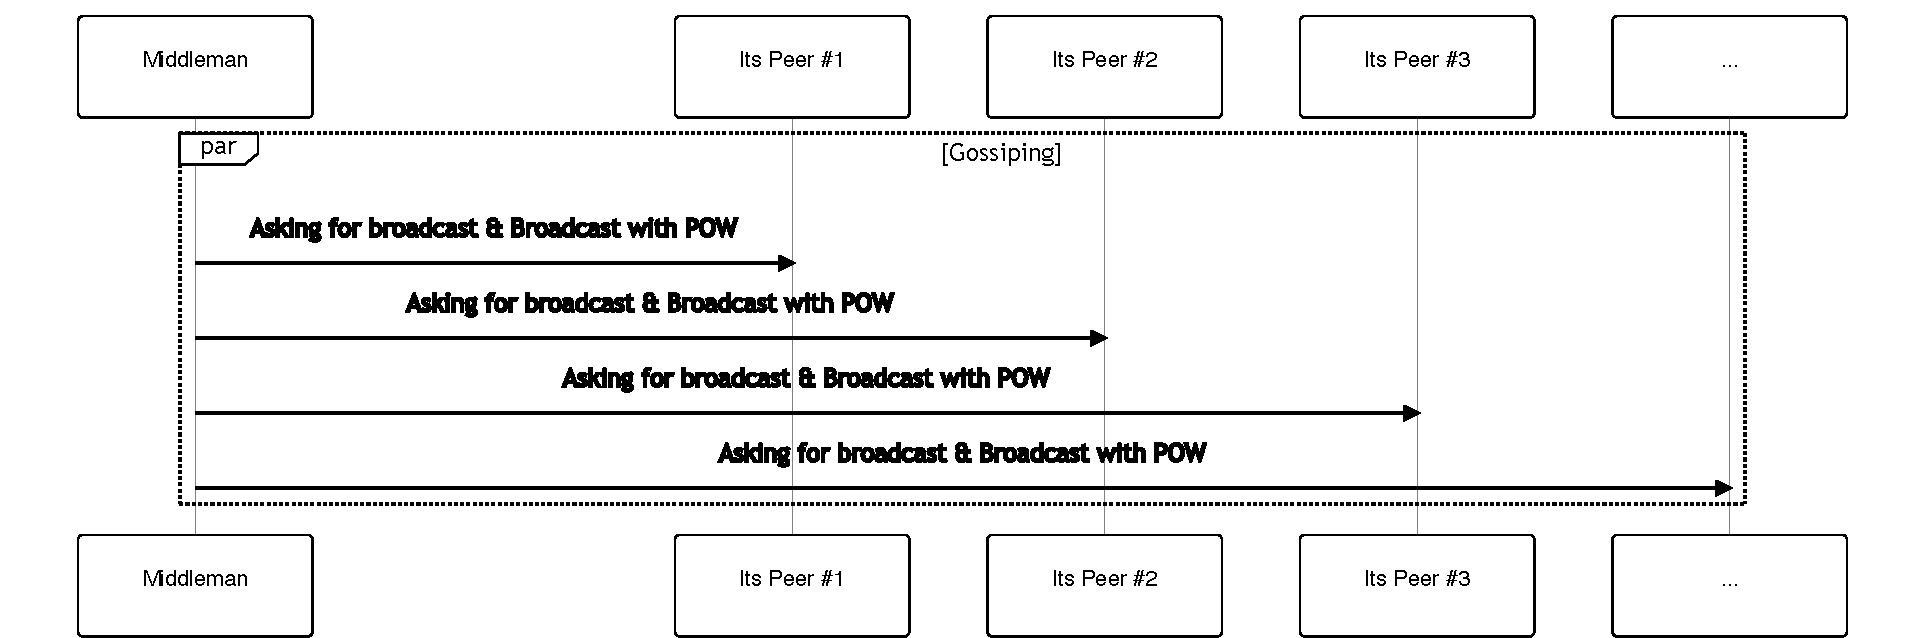
\includegraphics[scale=0.5]{BroadcastSequence.pdf}
	\caption{Broadcast Sequence}
	\label{fig:fr:broadcastsequence}
\end{figure}

\subsection{Lightning network, invoices, payments, preimages and payment-hashes}

Lightning network is a layer 2 network built on top of bitcoin network that allows for cheap and fast micropayments.
It is built around concept of channels. Once channel is opened (that usually means funding it with some amount of BTC), it can be used to issue the invoice and pay the invoce. Payment generates a proof. This idea is extended with cryptographic concept of preimage for payment hash in the following way:
\begin{enumerate}
	\item Invoice is issued by the issuer and as one of the fiels it contains specific payment hash. Payment hash is a hash of preimage that itself is a number known only to the invoice issuer at this moment and the payment-hash is the only thing that is exposed on the invoice.
	\item Payer is paing the invoice under condition of having preimage published by the issuer. In other words, the payment means that the invoice is paid if the issuer publish the preimage that has the payment-hash that was presented on the invoice.
\end{enumerate}

\begin{figure}
	\centering
	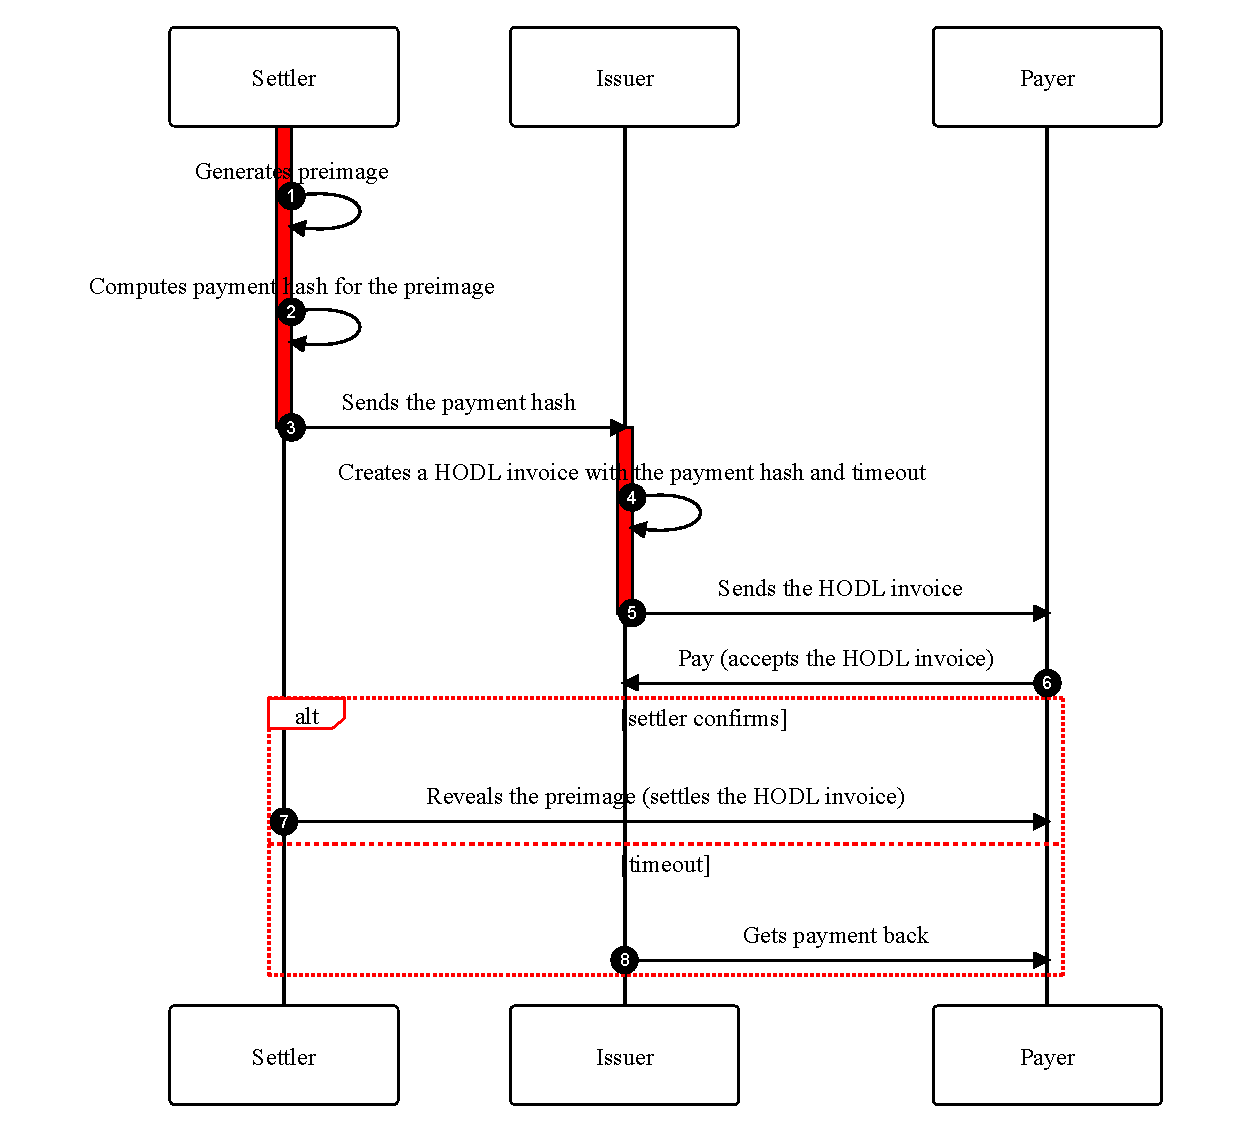
\includegraphics[scale=0.6]{LNDSequence.pdf}
	\caption{Lightning Network Sequence}
	\label{fig:fr:lndsequence}
\end{figure}

If one use cryptographic keys as a preimage in the scheme described above, one can think about this scheme as being secure, atomic micropayments in exchange for cryptographic keys.

Having a message that is encrypted with K different keys we can construct K invoices using separate key as a preimage and compute payment hash for each of the invoices. To decode the message payee need to pay all the invoices and obtain all the keys (preimages).

\subsection{Replying}
The node that is happy to accept the broadcasted message (replier) instead of broadcasting it further is replying it back. It is done with ResponseFrame that is sent back to the node that was the sender of the topic.


\begin{figure}
	\centering
	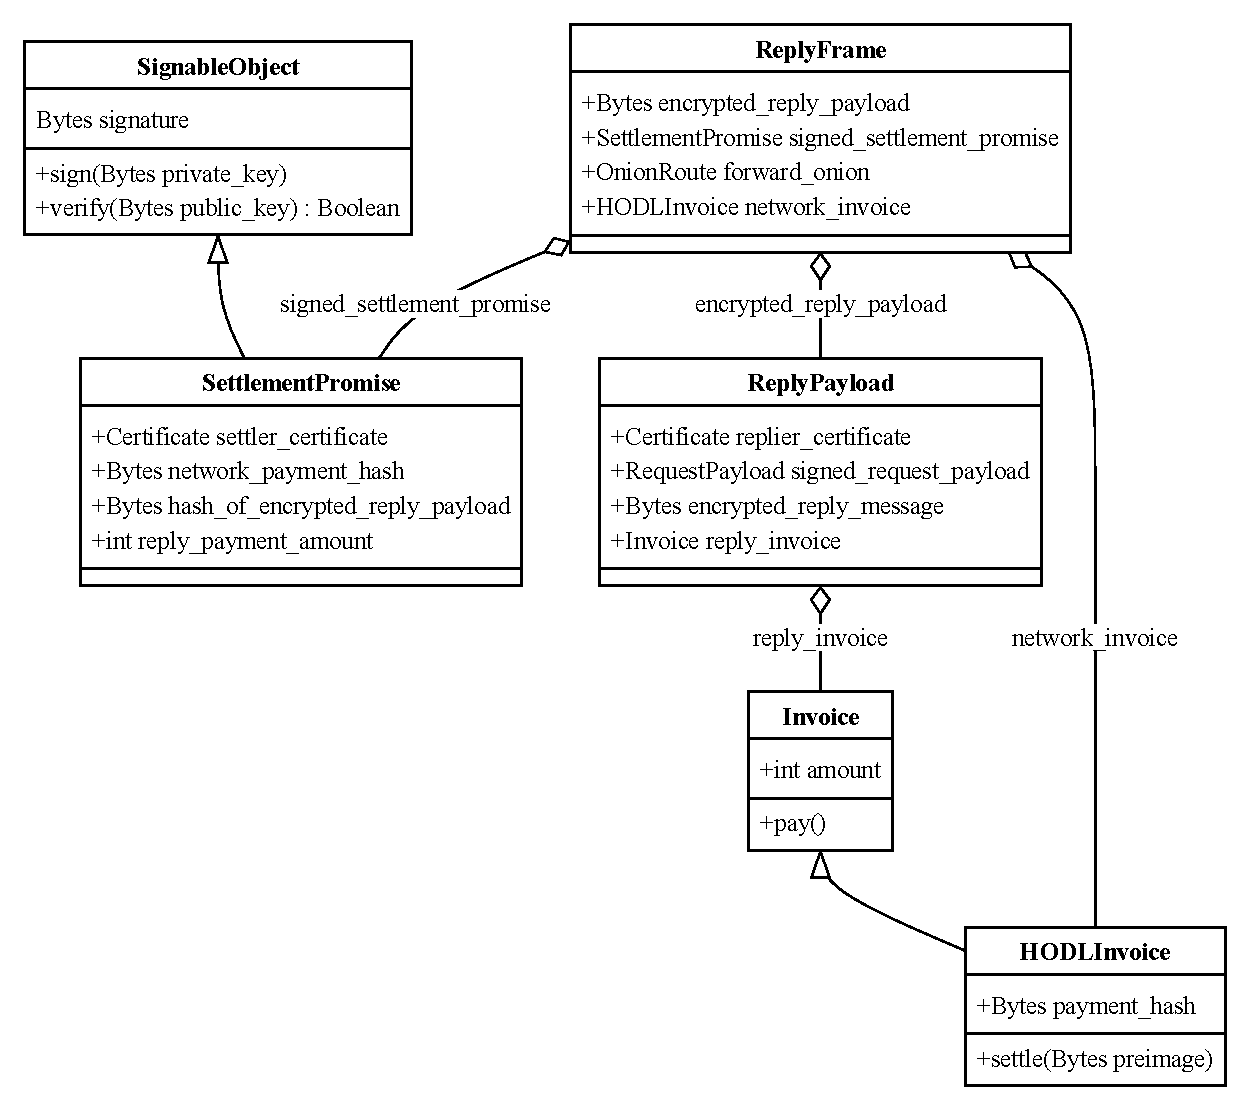
\includegraphics[scale=1.0]{ReplyFrame.pdf}
	\caption{Reply Frame}
	\label{fig:fr:replyframe}
\end{figure}

The replyier\_certificate has two meanings here:

\begin{enumerate}
	\item It allows the sender of the topic to identify that the gig contractor is a credible service provider by checking the certificate and verifing its "hard" certification (e.g. driving licence) with the specific certification authority being a trusted third party (e.g. government agency or specialised certification veryfier)
	\item It contains the replier public\_key that is used to verify the signature of the Reply Payload.
\end{enumerate}

The main part of the reply is the message that is encrypted so it can be used only after the sender (customer) will pay the network. The encryption is done by the replier and its correctness is verified by the network while traveling back to the sender. This is done in the following way:

\begin{enumerate}
	\item Replier encrypts the message with the sender public\_key that is a part of senders Certificate in the RequestPayload
	\item Replier geneates LND invoice that can be viewed by the sender and must be used to pay for the service after the service is delivered. Sender is not obligated to pay it if decides not to use the replier. On the other hand the invoice is signed by the replier and the replier cannot change it after the sender accepts the service to be provided by the replier.
	\item It generates N symmetric keys, where N is the number of elements of the routing\_payment\_instruction\_list, so for every instruction list we have a symmetric key. These symmetric keys will be used as preimages for generating all the invoices.
	\item It performs symmetric encryption using all the generated symmetric keys
	\item The encrypted message needs all the symmetric keys and the private key of the sender to be decrypted, making obligatory for the sender to obtain all the preimages, and therefore all the proofs of payments for all the invoices.
	\item For all the generated symmetric keys (preimages), the sender is computing payment hashes, so the network nodes can verify that the preimages are consistent with the hashes.
	\item All the preimages are encrypted with the public\_keys of the middleman that are about to generate invoices, so noone else is able to guess them. This computations togheter with payment hashes are stored in payment\_crypto\_instruction\_list.
	\item Request payload, encrypted message and payment\_crypto\_instruction\_list and are signed with the private key of the replier, so its integrity can be verified with replier Certificate
\end{enumerate}

The ReplyFrame contains Replier Certificate, ReplyPayload and additionally:

\begin{itemize}
	\item  forward onion
	\item  payment\_crypto\_instruction\_list
	\item  invoices
\end{itemize}

When replying the forward onion is simply a copy of the backward onion, then each of the middlemen is peeling one layer of the onion, using its private key and sending it to the node that is found there in the peel.

While traveling back, the ReplyFrame starts with empty list of invoces. Then each of the middleman is decrypting  its preimage from the payment\_crypto\_instruction\_list and is appending invoice with the hash equal to the specific preimage. This way when the frame reaches the source the preimage list is empty and contains all the invoices needed to be paid.

The source retrieving the Reply message pays all the invoices and this way it retrievies all the preimages that then are used to decrypt the message

\subsection{Payment errors}

If the one of invoices payment fails for some reason, it makes impossible for the payer to obtain its preimage and therefore decode the message even if all the other payments were succesful.

Fortunatelly gossip protocols do not prevent multpiple routes to reach the target, therefore the replier can reply multiple times for the same topic. This gives the sender a possibility to:

\begin{enumerate}
	\item select the cheapest route
	\item recover the payments that were already made in case if some of the other payments were unsuccesful. To implement this approach we need to make sure that the replier is using the same preimages for the same accounts when replying to multiple routes with the same topic. If this is true the sender can collect all the preimages that were paid and chose to use the other route with the maximum amount that was already paid to minimise the cost.
\end{enumerate}

[This concludes the protocol.]


\section{Discussion}

\subsection{Distributed Trust}

Certification Authority hierarchy is used commonly in the modern internet design however it is based on the idea of trusted 3rd parties. Having Certification Authorities that coexist in a free market helps with decentralization of trust.

The other approach for distributed trust is based on the idea of a track record. Track record means that the specific customer (sender) or gig-worker (replier) were already involved in series of successful transactions. This can be implemented using proof of payments that can be tracked back to the specific service being delivered.

The other one is based on the idea of reputation (transitive recommendations), so trustworthy participants are recommending other participants puting their reputation on a table.

\subsection{Mobile device connectivity issues}


Holepunching \cite{HolePunching}

Broken connection

\subsection{Attacks}
Here we are discussing common attacks that can be perfomed on the sweet-gossip network.


\begin{table}  
	\centering
	\begin{tabular}{ll}
		\toprule
		Attack         &   Sweet-Gossip defense \\
		\midrule
		Spam           & POW \\
		DDoS           & POW \\
		Silent         & Multibroadcast > 1 \\
		Chatterbox     & POW \\
		Sybil          & POW \\
		Eclipse        & Multibroadcast >1 \\
		Censorship     & - \\
		Convert Flash  & - \\
		\bottomrule
	\end{tabular}
	\label{tab:attacks}
	\caption{Attacks}
\end{table}


\subsubsection{The Silent Attack}
The adversary tries to distort the distribution of the gossipy nodes to cause propagation failure by failing to respond to the gossip protocol \cite{AdHocNet}. The same behaviour can be just a result of node failure that can happen naturally especially with mobile devices.

Multibroadcast > 1


\subsubsection{Chaterbox Attack}
A malicious node retransmits repeatedly the same message \cite{AdHocNet}.

\subsubsection{Sybil Attack}
This is the most common form of attack in P2P networks, since creating large numbers of identities is
generally cheap resource-wise, unless cryptographic puzzles are included as part of joining the system \cite{GossipSub}.

\subsubsection{Eclipse Attack}
This attack can be carried out against a single victim or the whole network. The objective is to
silence the victim by refusing to propagate messages from it or to distort its view by delaying message propagation towards it \cite{GossipSub}.
Here the attact can be performed agains specific Certification Authority

\subsubsection{Censorship Attack}
Sybils seek to establish themselves in the mesh and propagate all messages except those published by the target peer. In contrast to the Eclipse Attack, in the Censorship Attack Sybils appear to behave properly
from all vantage points, but hairpin-drop the victim's messages. The objective of the attacker is to censor the target and prevent its messages from reaching the rest of the network \cite{GossipSub}.

\subsubsection{Covert Flash Attack}
In the Covert Flash Attack, Sybils connect to the network but behave properly for some time in order to build up score. Then, they execute a coordinated attack whereby they stop propagating messages altogether in an attempt to completely disrupt the network. The attack is difficult to identify before the attackers turn malicious as they behave properly up to that point and build a good profile \cite{GossipSub}.

\section{Supporting Services}

\subsection{KYC services as Certification Authorities}

\subsection{Push notification servers}

\subsection{Map servers}

\section{Applications}

Sweet-Gossip Protocol is an enabler for building P2P apps.


\section{Public Key}
This is the Public Key (GPG) of Sonof Satoshi.
\label{gpgkey}
\begin{small}
\begin{verbatim}
-----BEGIN PGP PUBLIC KEY BLOCK-----

mI0EY8pcpgEEAN+bUaEdg+ylWkdNc6U9LNkWb4ii0Neay4kUyU2NntHMlFAZPNSC
wxJ8PlbrQnOGeeGNyfZtjZKTSn0Jor5YT4pHNlubGFj3/BrihJCBRSJ878qO2ct9
4RJXiNADVg1w3jRKRrk1CimmmL7VVK7oFZHd0311+8r/qIT4WNOITydNABEBAAG0
MVNvbm9mIFNhdG9zaGkgPHNvbm9mLnNhdG9zaGlAZG9udHRydXN0dmVyaWZ5Lm9y
Zz6I0QQTAQgAOxYhBIaALVutWo8Bqg5fDYtkf+QR5XMgBQJjylymAhsDBQsJCAcC
AiICBhUKCQgLAgQWAgMBAh4HAheAAAoJEItkf+QR5XMg2PYEAMcEB370PgxAaV+e
Kt458OPymI/rZOWO6Cm9E6BqMdNqNx7d4udxbQYutkUr1xhLmLH1JTxJwFhe3oMv
/3MUjm/VjIYrdnXAhHqvZA3502AyiWEQ66OQ9whj57PY04YYcBZP/NDe4QuoUX9r
b3XzYIeJcqHUNg0zjjQJQ7bU7gcwuI0EY8pcpgEEAK/nkFTpiOiGtUI1RqWD46HA
nH7wTVXy2BVwHefRiDHz2hGgQiHXF6EU8mk9F2SVBjOTBNHGAwvXssT97Y8jiq6i
vJosx7VtolxBEDRL1PFMOH4whwu1rjDg8QR3KPkB3kMcXvD9ZHIB6FspVvhx2/Jk
V+PKLQ0ThhQITxFIKz4nABEBAAGItgQYAQgAIBYhBIaALVutWo8Bqg5fDYtkf+QR
5XMgBQJjylymAhsMAAoJEItkf+QR5XMgRngD/0GbcDFoL8hqppvuBuXBLHJVMLGh
fF/3fZyd1ZkjE+Il/LX5G/WSsLcAm/dmAVd8L1zat3PvdL57RHY06BEE4kdDEo8m
DlZ8SycI1yGaSS8DdGCMaAFLzOxrJgER3NnXxg7BxCfREcUTawq1CEO1QYx/71ib
GoTF/wPiCY/JQ1Ed
=Ei5q
-----END PGP PUBLIC KEY BLOCK-----
\end{verbatim}
\end{small}


\bibliographystyle{abbrv}
\bibliography{references}  

\end{document}
